\section{Edge Execution and Compression}
\label{sec:edge}

\begin{figure}[!t]
\centering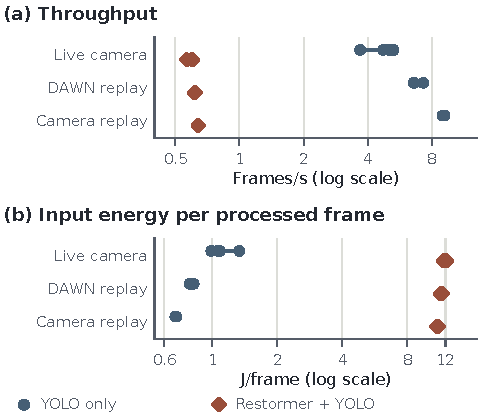
\includegraphics[width=\linewidth]{figures/nano_runtime.pdf}
\caption{Original Jetson Nano throughput and board input energy. Each point is one weather condition. The lines span conditions within a workload. Live application FPS and replay FPS have different timing boundaries. Energy uses integrated board input power divided by processed frames.}
\label{fig:nano-runtime}
\end{figure}

\paragraph{Measured Nano execution.}
Figure~\ref{fig:nano-runtime} separates live, labelled replay, and saved-camera replay. In DAWN replay, YOLO alone reaches 6.55--7.28 FPS with median pipeline latency of 129.2--147.2\,ms. Adding the $128\times128$ restorer yields 0.61--0.62 FPS and 1,596.7--1,619.6\,ms. Board input energy rises from 0.78--0.82 to 11.35--11.59\,J/frame, about 14--15 times more across weather subsets. The live cascade runs at 0.57--0.60 FPS. Live throughput includes capture, weather generation, display, and application overhead. Replay isolates the processing path. Power integrates the board input rail without subtracting idle power. Short, single-run windows constrain runtime and energy estimates (Appendix~\ref{app:hardware}).

\begin{figure*}[t]
\centering
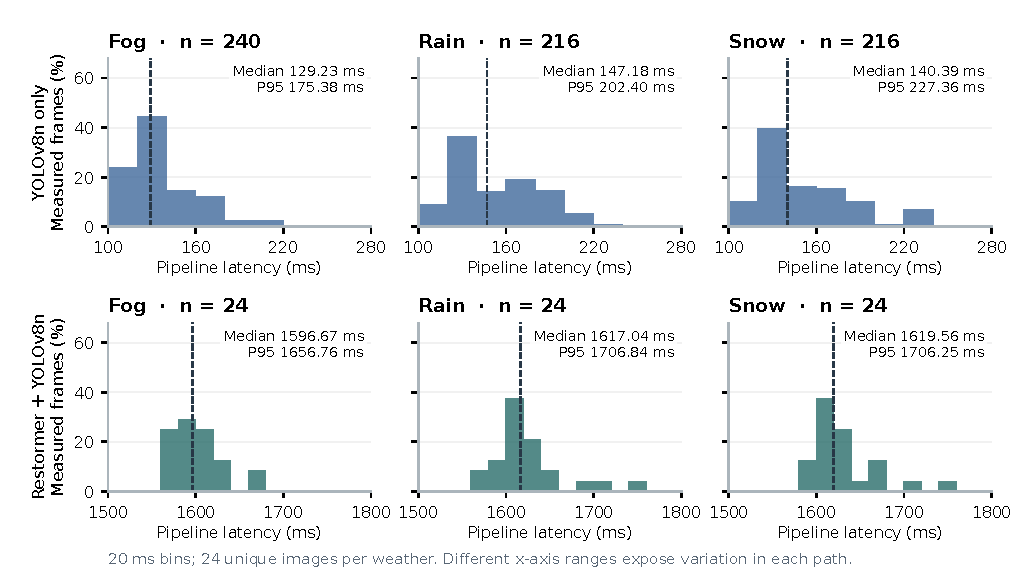
\includegraphics[width=.98\textwidth]{figures/nano_pipeline_latency_histograms.pdf}
\caption{Measured per-frame pipeline latency on the Jetson Nano for YOLOv8n alone and Restormer ($128\!\times\!128$ restoration canvas) followed by YOLOv8n. The saved labelled replay uses 24 unique images per weather and five excluded warm-up frames. The raw path repeats the images to record 240/216/216 timed frames; the restored path records 24 per weather, with each window lasting at least 30 seconds. Histograms use 20 ms bins and normalize each run to 100\%; dashed lines mark medians. The two rows deliberately use different latency ranges. Timing covers synchronized restoration/resize and detector preprocessing, inference and NMS; capture, decoding, weather synthesis, scoring and preview are excluded.}
\label{fig:nano-latency-histograms}
\end{figure*}


Figure~\ref{fig:nano-latency-histograms} shows the full measured latency
distributions. Median raw pipeline latency is 129.23--147.18\,ms, compared
with 1,596.67--1,619.56\,ms after adding Restormer. The observations repeat
images within the recorded runs; they are not independent repeated trials
or live-camera timing.

\paragraph{Conversion and deployment.}
The measured cascade uses FP32 YOLOv8n and a mixed FP16/FP32 Restormer on the original 4\,GB Jetson Nano with TensorRT 8.2.1.8. Its detector and restorer pass three and four numerical fixtures, respectively. Lower-precision weights can reduce storage and memory traffic when the runtime packs and executes them. The separate 8-bit weight grid retains FP32 execution and storage at 105,748,439 bytes. Fog and smoke exceed its output RMSE limit at $6.18\times10^{-3}$ and $4.64\times10^{-3}$. The 8-bit candidate and pruning controls remain offline screens (Section~\ref{app:quant}).

\subsection{Memory observations}
\begin{figure*}[t]
\centering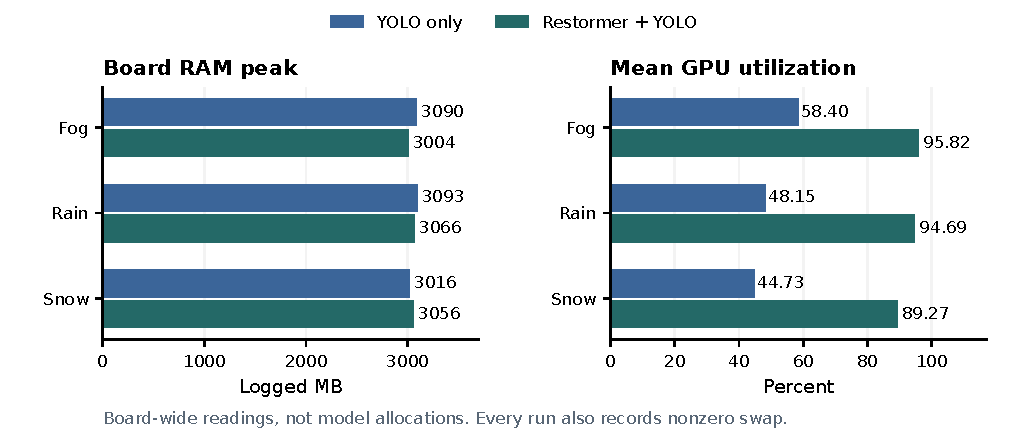
\includegraphics[width=.98\linewidth]{figures/nano_resources.pdf}
\caption{Resource observations from the completed Nano replay. The cascade uses the GPU more heavily, while board-wide RAM peaks remain near 3 GB. These logged peaks include other board processes and do not measure the restorer's isolated allocation.}
\label{fig:nano-resources}
\end{figure*}
\begin{table}[t]
\centering\small
\caption{Recorded board memory and GPU utilization during labelled DAWN replay. RAM and swap are board-wide peaks in the logged MB units, not isolated model allocations.}
\label{tab:memory}
\begin{tabular}{@{}llrrr@{}}\toprule
Weather & Path & RAM & Swap & GPU (\%)\\\midrule
Fog & YOLO & 3090 & 1384 & 58.4\\
Fog & Cascade & 3004 & 1368 & 95.8\\
Rain & YOLO & 3093 & 1384 & 48.1\\
Rain & Cascade & 3066 & 1378 & 94.7\\
Snow & YOLO & 3016 & 1384 & 44.7\\
Snow & Cascade & 3056 & 1382 & 89.3\\
\bottomrule
\end{tabular}
\end{table}

Figure~\ref{fig:nano-resources} and Table~\ref{tab:memory} supplement timing with the recorded memory context.
All six labelled replay runs report nonzero swap. Mean GPU utilization is
89.3--95.8\% for the cascade and 44.7--58.4\% for YOLO alone. These are
whole-board observations from the short workloads; they do not isolate the
restorer's allocation or prove that swap caused the latency difference.

\subsection{Weight Discretization and Pruning}
\label{app:quant}
\subsubsection{Weight-grid transformation}

The ONNX adapter identifies convolution initializers from graph edges. It preserves two boundary tensors and discretizes 272 convolution tensors, including attention projections and feed-forward convolutions. Activations, matrix attention, normalization, storage, and runtime remain FP32 (Fig.~\ref{fig:weight-grid}).

For each output channel of $m$ weights, the order statistic is $k=\max(1,\operatorname{round}(0.9995m))$. With $a$ the $k$th absolute weight magnitude, the scale is $s=\max(a,10^{-8})/127$. The zero point is zero, and PyTorch rounding gives
\begin{equation}
q=\clip(\operatorname{round}(w/s),-128,127),\qquad \tilde w=sq.
\end{equation}
Small kernels may select their maximum magnitude. The reconstructed $\tilde w$ replaces the FP32 initializer. Both serialized ONNX graphs occupy 105,748,439 bytes.

\subsubsection{Quality retention and output agreement}
For the normalized $[-1,1]$ output tensors $z$ and $\tilde z$, agreement uses
\begin{equation}
e_{\rm rms}=\sqrt{\tfrac1N\sum_j(\tilde z_j-z_j)^2},
\quad e_{\infty}=\max_j|\tilde z_j-z_j|.
\end{equation}
Quality is evaluated on cropped RGB $[0,1]$ against the clean target. RGB PSNR uses a $10^{-12}$ MSE floor. SSIM uses a uniform $7\times7$ window, sample covariance, and constants $0.01^2$ and $0.03^2$. The four-fixture gate requires $\Delta\mathrm{PSNR}\geq-0.1$ dB, $\Delta\mathrm{SSIM}\geq-0.001$, $e_{\rm rms}\leq0.004$, and $e_\infty\leq0.05$, with finite outputs and matching shapes. Fog and smoke fail the RMSE condition.

\FloatBarrier
\begin{figure*}[!t]
\centering\begingroup
\setbox0=\hbox{\resizebox{\textwidth}{!}{\begin{tikzpicture}[
  x=1cm,y=1cm,
  op/.style={draw=aegisgray!40,fill=aegishead,text width=3.56cm,
    minimum height=1.18cm,inner sep=4pt,align=center,font=\small},
  check/.style={draw=aegisblue!30,fill=aegisbest,text width=6.85cm,
    minimum height=1.08cm,inner sep=4pt,align=center,font=\small},
  flow/.style={-{Latex[length=2.0mm]},aegisblue,line width=.76pt}]
\node[op] (weights) at (1.96,0) {\textbf{FP32 convolution}\\weights by output channel};
\node[op] (scale) at (6.35,0) {\textbf{Scale from magnitudes}\\99.95th-percentile rank};
\node[op] (grid) at (10.74,0) {\textbf{Round and clamp}\\Signed levels $[-128,127]$};
\node[op] (onnx) at (15.13,0) {\textbf{Reconstruct as FP32}\\$\tilde w=sq$ in the ONNX graph};
\draw[flow] (weights) -- (scale);
\draw[flow] (scale) -- (grid);
\draw[flow] (grid) -- (onnx);
\node[check] (reference) at (4.27,-1.99) {\textbf{Quality against clean targets}\\Valid RGB pixels in $[0,1]$\\Change in PSNR and SSIM};
\node[check] (output) at (12.83,-1.99) {\textbf{Agreement against the FP32 baseline}\\Normalized full output tensor\\RMSE and maximum absolute error};
\coordinate (branch) at (15.13,-.94);
\draw[aegisblue,line width=.76pt] (onnx.south) -- (branch);
\draw[flow] (branch) -| (reference.north);
\draw[flow] (branch) -| (output.north);
\end{tikzpicture}
}}%
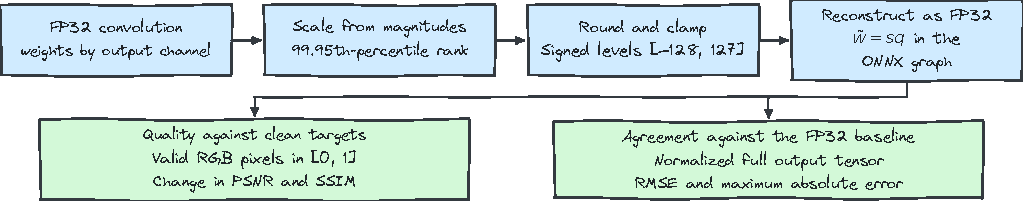
\includegraphics[width=\wd0,height=\ht0]{figures/weight_grid_workflow_excalidraw.pdf}%
\endgroup
\caption{Weight-grid screen. Convolution weights are discretized per output channel and reconstructed in FP32. Clean-target quality uses cropped valid RGB pixels. Numerical agreement uses the full normalized output tensor.}
\label{fig:weight-grid}
\end{figure*}

\begin{table}[!t]
\centering\small
\caption{Absolute clean-reference quality and maximum output error for the 8-bit weight grid. SSIM and output error are scaled by 100 for display.}
\begin{tabular}{@{}lrrrr@{}}\toprule
Weather & Base PSNR & Grid PSNR & SSIM $\times100$ & $100e_\infty$\\\midrule
Rain &34.28&34.37&95.82&2.45\\
Fog &24.36&24.38&88.93&4.67\\
Snow &36.96&36.89&97.39&2.54\\
Smoke &21.84&21.87&83.96&2.14\\\bottomrule
\end{tabular}
\end{table}

\begin{figure*}[!t]
\centering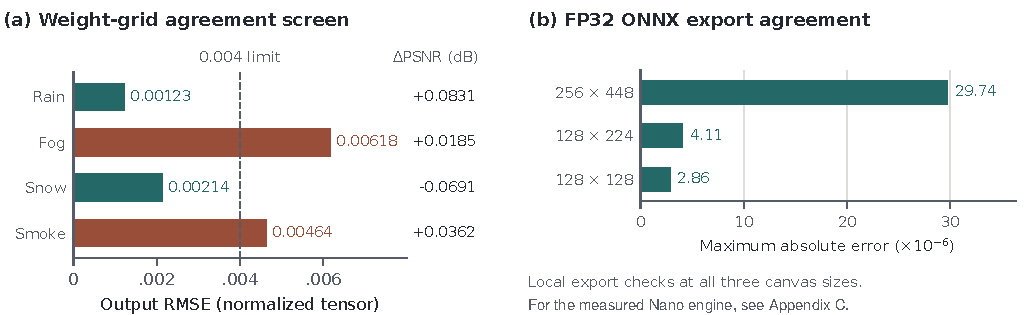
\includegraphics[width=\textwidth]{figures/edge_acceptance_current.pdf}
\caption{Offline numerical screens. \textbf{(a)} Weight-grid RMSE on normalized outputs, alongside clean-target PSNR changes. Fog and smoke exceed the 0.004 gate. \textbf{(b)} Local FP32 PyTorch--ONNX agreement by canvas size. Earlier build observations describe the path to the separately evaluated mixed engine in Appendix~\ref{app:hardware}.}
\label{fig:edge}
\end{figure*}

\subsubsection{Linear-only conversion and pruning controls}
A dynamic conversion restricted to linear modules finds no eligible layers. It converts zero modules and preserves all state tensors. Restormer uses convolutions for its projection layers.

\begin{figure}[!t]
\centering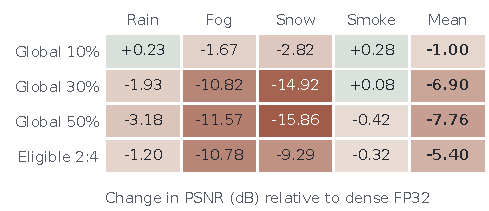
\includegraphics[width=\linewidth]{figures/pruning_screen_matrix.pdf}
\caption{Pruning changes in PSNR on four fixtures. The mean weights fixtures equally. Every masked variant fails the retention screen.}
\label{fig:pruning-screen}
\end{figure}
Global magnitude pruning masks convolution weights without retraining. The eligible 2:4 mask produces 39.68\% sparsity over the tested population of 26,096,544 convolution weights. All masked state dictionaries remain 104,696,534 bytes, with explicit zeros in dense tensors. Figure~\ref{fig:pruning-screen} shows the per-fixture quality losses. At 10\% global sparsity, fog and snow fail both quality criteria, and smoke fails its SSIM criterion.

